%% LyX 2.2.0 created this file.  For more info, see http://www.lyx.org/.
%% Do not edit unless you really know what you are doing.
\documentclass[11pt,american]{beamer}
\usepackage{lmodern}
\renewcommand{\sfdefault}{lmss}
\renewcommand{\ttdefault}{lmtt}
\usepackage[T1]{fontenc}
\usepackage[latin9]{inputenc}
\setcounter{secnumdepth}{3}
\setcounter{tocdepth}{3}
\usepackage{textcomp}
\usepackage{amssymb}
\usepackage{graphicx}

\makeatletter

%%%%%%%%%%%%%%%%%%%%%%%%%%%%%% LyX specific LaTeX commands.
\pdfpageheight\paperheight
\pdfpagewidth\paperwidth


%%%%%%%%%%%%%%%%%%%%%%%%%%%%%% Textclass specific LaTeX commands.
 % this default might be overridden by plain title style
 \newcommand\makebeamertitle{\frame{\maketitle}}%
 % (ERT) argument for the TOC
 \AtBeginDocument{%
   \let\origtableofcontents=\tableofcontents
   \def\tableofcontents{\@ifnextchar[{\origtableofcontents}{\gobbletableofcontents}}
   \def\gobbletableofcontents#1{\origtableofcontents}
 }
 % plain title style, override default
 \renewcommand\makebeamertitle{\frame[plain]{\maketitle}}%

\@ifundefined{date}{}{\date{}}
%%%%%%%%%%%%%%%%%%%%%%%%%%%%%% User specified LaTeX commands.
\usepackage{microtype}
\usetheme{Frankfurt}
\definecolor{blue1}{RGB}{51,51,179}
\definecolor{blue2}{RGB}{0,0,204}
\definecolor{blue3}{RGB}{0,0,153}
\setbeamercolor{author in head/foot}{fg=white, bg=blue3}
\setbeamercolor{title in head/foot}{fg=white, bg=blue2}
\setbeamercolor{date in head/foot}{fg=white, bg=blue1}
\useoutertheme{split}
\setbeamertemplate{navigation symbols}{}
\setbeamertemplate{footline}
{
  \leavevmode%
  \hbox{%
  \begin{beamercolorbox}[wd=.333333\paperwidth,ht=2.25ex,dp=1ex,center]{author in head/foot}%
    \usebeamerfont{author in head/foot}\insertshortauthor~~\beamer@ifempty{\insertshortinstitute}{}{(\insertshortinstitute)}
  \end{beamercolorbox}%
  \begin{beamercolorbox}[wd=.333333\paperwidth,ht=2.25ex,dp=1ex,center]{title in head/foot}%
    \usebeamerfont{title in head/foot}\insertshorttitle
  \end{beamercolorbox}%
  \begin{beamercolorbox}[wd=.333333\paperwidth,ht=2.25ex,dp=1ex,right]{date in head/foot}%
    \usebeamerfont{date in head/foot}\insertshortdate{}\hspace*{2em}
    \insertframenumber{} / \inserttotalframenumber\hspace*{2ex} 
  \end{beamercolorbox}}%
  \vskip0pt%
}
\usepackage[absolute,overlay]{textpos}
\setlength{\TPHorizModule}{1mm}
  \setlength{\TPVertModule}{1mm}
\newcommand\Fontvi{\fontsize{8}{12}\selectfont}

\makeatother

\usepackage{babel}
\begin{document}

\title[Progetto SE II]{Progetto di Ingegneria del Software II }

\author[Scorsolini, Semeria, Vanoni]{Philippe Scorsolini,\\
Lorenzo Semeria,\\
Gabriele Vanoni}

\institute[PoliMi]{Politecnico di Milano}

\date{6 Marzo 2017}
\makebeamertitle
\begin{frame}{Indice}

\tableofcontents{}
\end{frame}

\section{Introduzione}
\begin{frame}{PowerEnJoy: caratteristiche principali}

\pause
\begin{itemize}
\item Servizio di Car Sharing di auto elettriche \pause
\item Prenotazione tramite smartphone \pause
\item Possibilit� di iniziare e terminare il noleggio solo all'interno di
zone predefinite \pause
\item Possibilit� di ottenere sconti in base ad alcuni parametri (numero
di passeggeri, termine noleggio in una stazione di ricarica)
\end{itemize}
\end{frame}

\section{Analisi dei requisiti e specifica}

\subsection{Requisiti Funzionali}
\begin{frame}[plain]
\begin{center}
\textbf{\Large{}Analisi dei requisiti}
\par\end{center}{\Large \par}

\end{frame}
\begin{frame}{I Goal}

Identificati\textbf{ 11 Goal} e un totale di \textbf{60 Requisiti}

I Goal possono essere suddivisi in tre macrogruppi:
\begin{itemize}
\item \textbf{Gestione utenti}
\item \textbf{Gestione auto}
\item \textbf{Utilizzo del Servizio}
\end{itemize}
\end{frame}
%
\begin{frame}{Gestione utenti}

Le caratteristiche e i requisiti della gestione utenti venogono definiti
dai primi 3 goal: \pause
\begin{itemize}
\item G1: \textbf{Registrazione} Utenti
\begin{itemize}
\item Sono necesarie email e patente valide. Il metodo di pagamento viene
aggiunto successivamente \pause
\end{itemize}
\item G2: \textbf{Login} utente
\begin{itemize}
\item I requisiti definiscono le caratteristiche principali di questo goal,
ad esempio la necessit� di inserire la combinazione corretta di username
e password \pause
\end{itemize}
\item G3: \textbf{Modifica} del profilo
\begin{itemize}
\item � possibile effettuare ogni modifica a condizione che i nuovi dati
inseriti siano validi 
\end{itemize}
\end{itemize}
\end{frame}
%
\begin{frame}{Gestione auto}

La gestione delle auto � fortemente collegata con l'utilizzo del servizio,
tra i goal principali possiamo individuare i seguenti. \pause
\begin{itemize}
\item G4: Mostrare le \textbf{informazioni} aggiornate sulle auto
\begin{itemize}
\item Le auto mantengono il sistema aggiornato sulla propria posizione e
carica. \pause
\end{itemize}
\item G6: Permettere lo \textbf{sblocco} dell'auto
\begin{itemize}
\item L'auto viene sbloccata dopo che il sistema conferma che l'utente �
nei pressi dell'auto
\end{itemize}
\end{itemize}
\end{frame}
%
\begin{frame}{Utilizzo del Servizio}

Le modalit� e i requisiti relativi all'utilizzo del servizio costituiscono
la maggior parte dei goal che abbiamo identificato. Tra i principali:
\pause
\begin{itemize}
\item G5/G6: \textbf{Prenotazione} e \textbf{sblocco} dell'auto prenotata\pause
\begin{itemize}
\item Azione riservata agli utenti abilitati. \pause
\item Comportamento nel caso in cui l'auto non venga sbloccata o messa in
moto in tempo. \pause
\end{itemize}
\item G7: Calcolo della \textbf{tariffa \pause}
\begin{itemize}
\item La tariffa viene calcolata tenendo conto di tutti i modificatori (sconti
o sovrapprezzi) e del tempo di utilizzo. \pause
\item Per alcuni casi particolari � stato previsto un comportamento ad hoc
\pause
\end{itemize}
\item G9: \textbf{Pagamento} della tariffa\pause
\begin{itemize}
\item Il pagamento viene effettuato immediatamente al termine del noleggio\pause
\item In caso di fallimento (metodo non pi� valido) l'utente viene notificato
e il suo account temporaneamente disabilitato. 
\end{itemize}
\end{itemize}
\end{frame}
%

\subsection{Requisiti non funzionali}
\begin{frame}{Requisiti non funzionali}
\begin{itemize}
\item Le applicazioni per gli utenti devono essere \textbf{user friendly
}\pause
\item Il sistema deve essere \textbf{disponibile sempre} (giorno e notte)\pause
\item Il sistema deve essere facilmente \textbf{scalabile} in caso di crescita\pause
\item I dati personali devono essere salvati in modo \textbf{sicuro} e nel
rispetto delle norme \pause
\item � fondamentale che il sistema sia ben protetto da attacchi per prevenire,
ad esempio, il furto di auto
\end{itemize}
\end{frame}
%
\begin{frame}{Soluzioni di alcuni casi ambigui }

In alcuni casi quanto scritto nella consegna non era del tutto esaustivo
dei possibili scenari, per cui abbiamo qualora necessario deciso come
gestire le singole eccezioni, ad esempio: \pause
\begin{itemize}
\item Il ``Problema IKEA'': \pause abbiamo deciso di permettere agli
utenti di ``parcheggiare'' nel senso comune del termine, ovvero
continuando a pagare per l'auto, se si trovano fuori dalle zone in
cui � possibile terminare il noleggio. (A12)\pause
\item Apertura delle portiere senza accensione: \pause dopo un breve periodo
di tempo il sistema chiede all'utente di confermare di star bene,
in caso contrario un Operatore si reca a verificare che non ci siano
problemi (ad esempio un malessere dell'utente). Altrimenti, trascorso
il tempo massimo di prenotazione, inizia a pagare la tariffa di utilizzo.
(R30 e R31)
\end{itemize}
\end{frame}

\subsection[Alloy]{Modellazione in Alloy}
\begin{frame}[plain]
\begin{center}
\textbf{\Large{}Modellazione in Alloy}
\par\end{center}{\Large \par}

\end{frame}
%
\begin{frame}{Il modello statico}

Abbiamo scelto di modellare in \textbf{Alloy} questa parte del nostro
\textbf{sistema}.

\medskip{}

\begin{center}
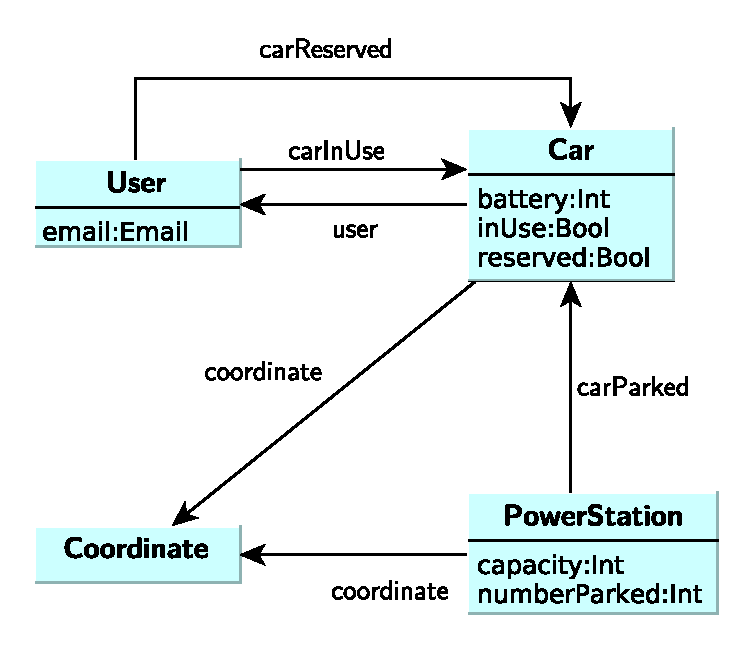
\includegraphics[scale=0.58]{classDiagram}
\par\end{center}

\end{frame}
%
\begin{frame}{Uno dei mondi possibili}

\begin{textblock}{100}(10,15)Questo � uno dei possibili output generati
dal solver di \textbf{Alloy}.\end{textblock}
\begin{center}
\begin{textblock}{100}(5,20)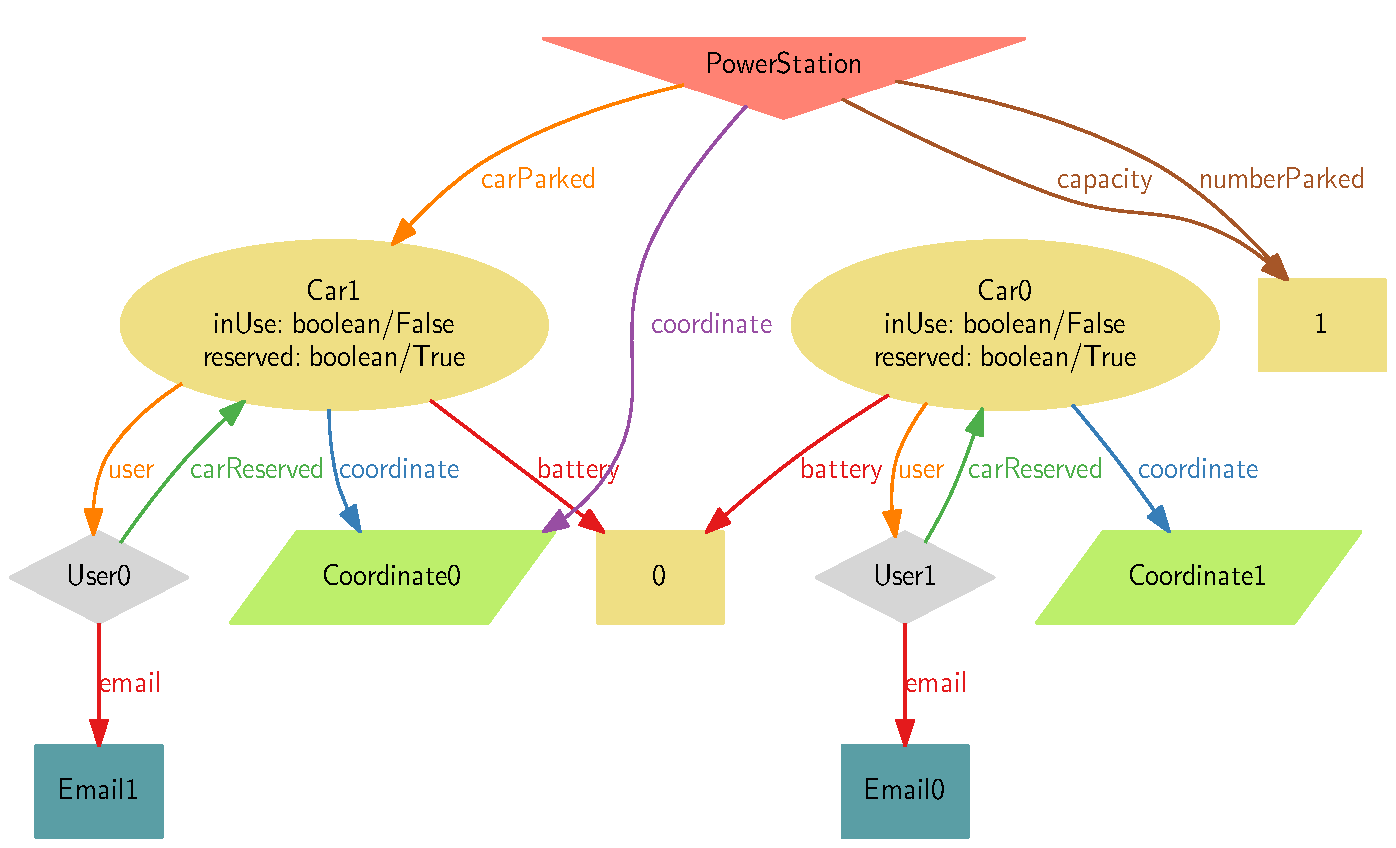
\includegraphics[scale=0.48]{showStatic}\end{textblock}
\par\end{center}

\end{frame}
%
\begin{frame}{Il modello dinamico}

\begin{textblock}{100}(10,15)Queste \textbf{azioni} sono state modellate
in Alloy come \textit{predicati}.\end{textblock}

\begin{textblock}{200}(5,25)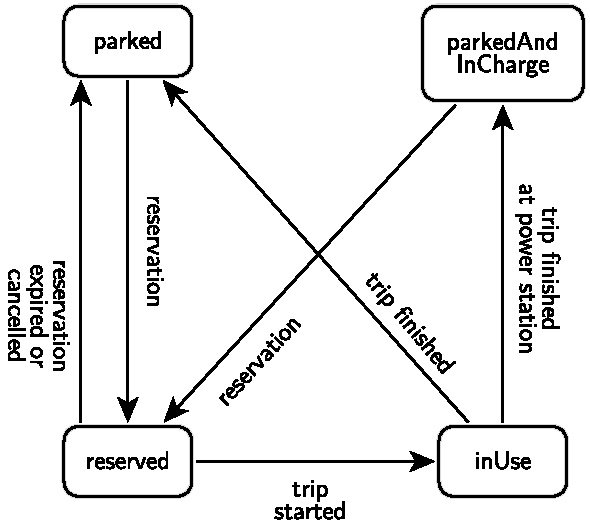
\includegraphics[scale=0.58]{stateDiagramCar}\hspace{1cm}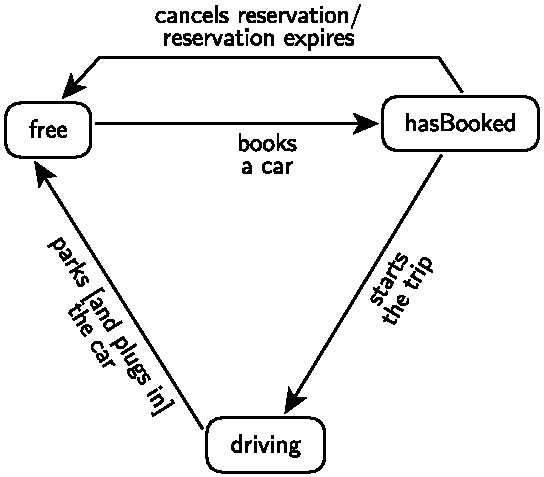
\includegraphics[scale=0.58]{stateDiagramUser}\end{textblock}
\end{frame}
%
\begin{frame}{Azione - prenotazione dell'auto}
\begin{center}
\begin{textblock}{100}(5,20)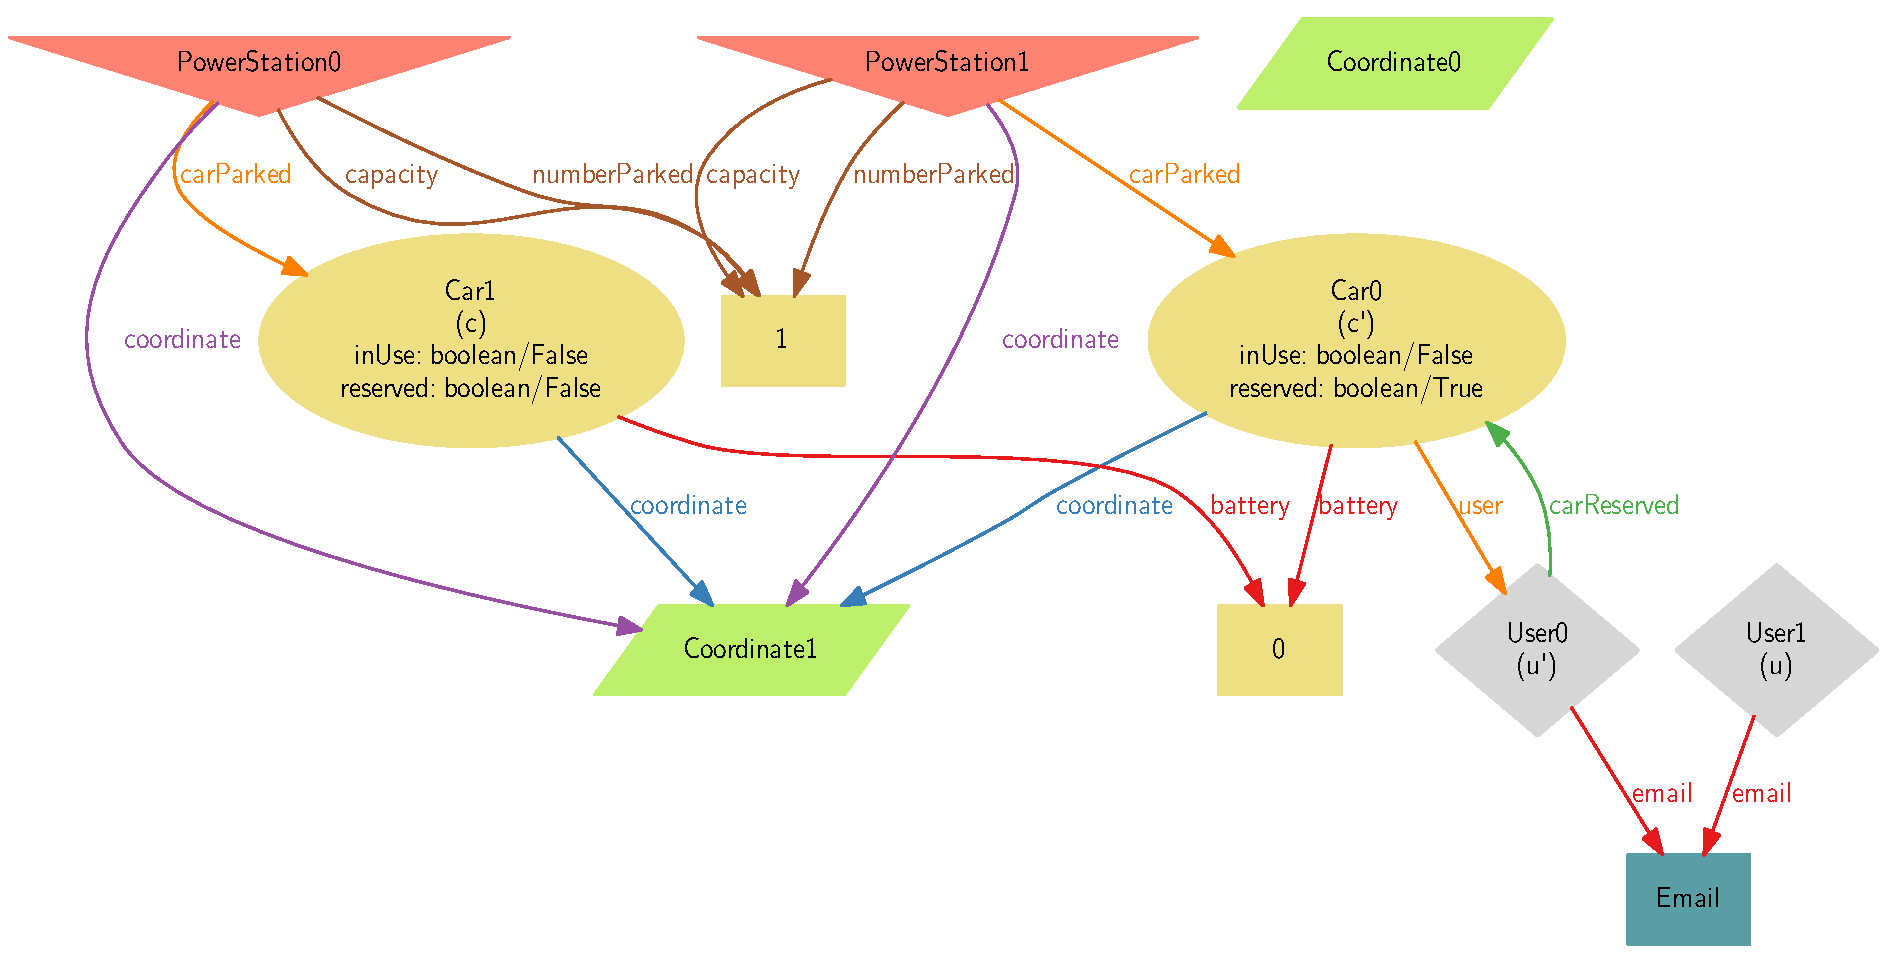
\includegraphics[scale=0.38]{reserveCar}\end{textblock}
\par\end{center}

\end{frame}
%
\begin{frame}{Azione - inizio del viaggio}
\begin{center}
\begin{textblock}{100}(5,15)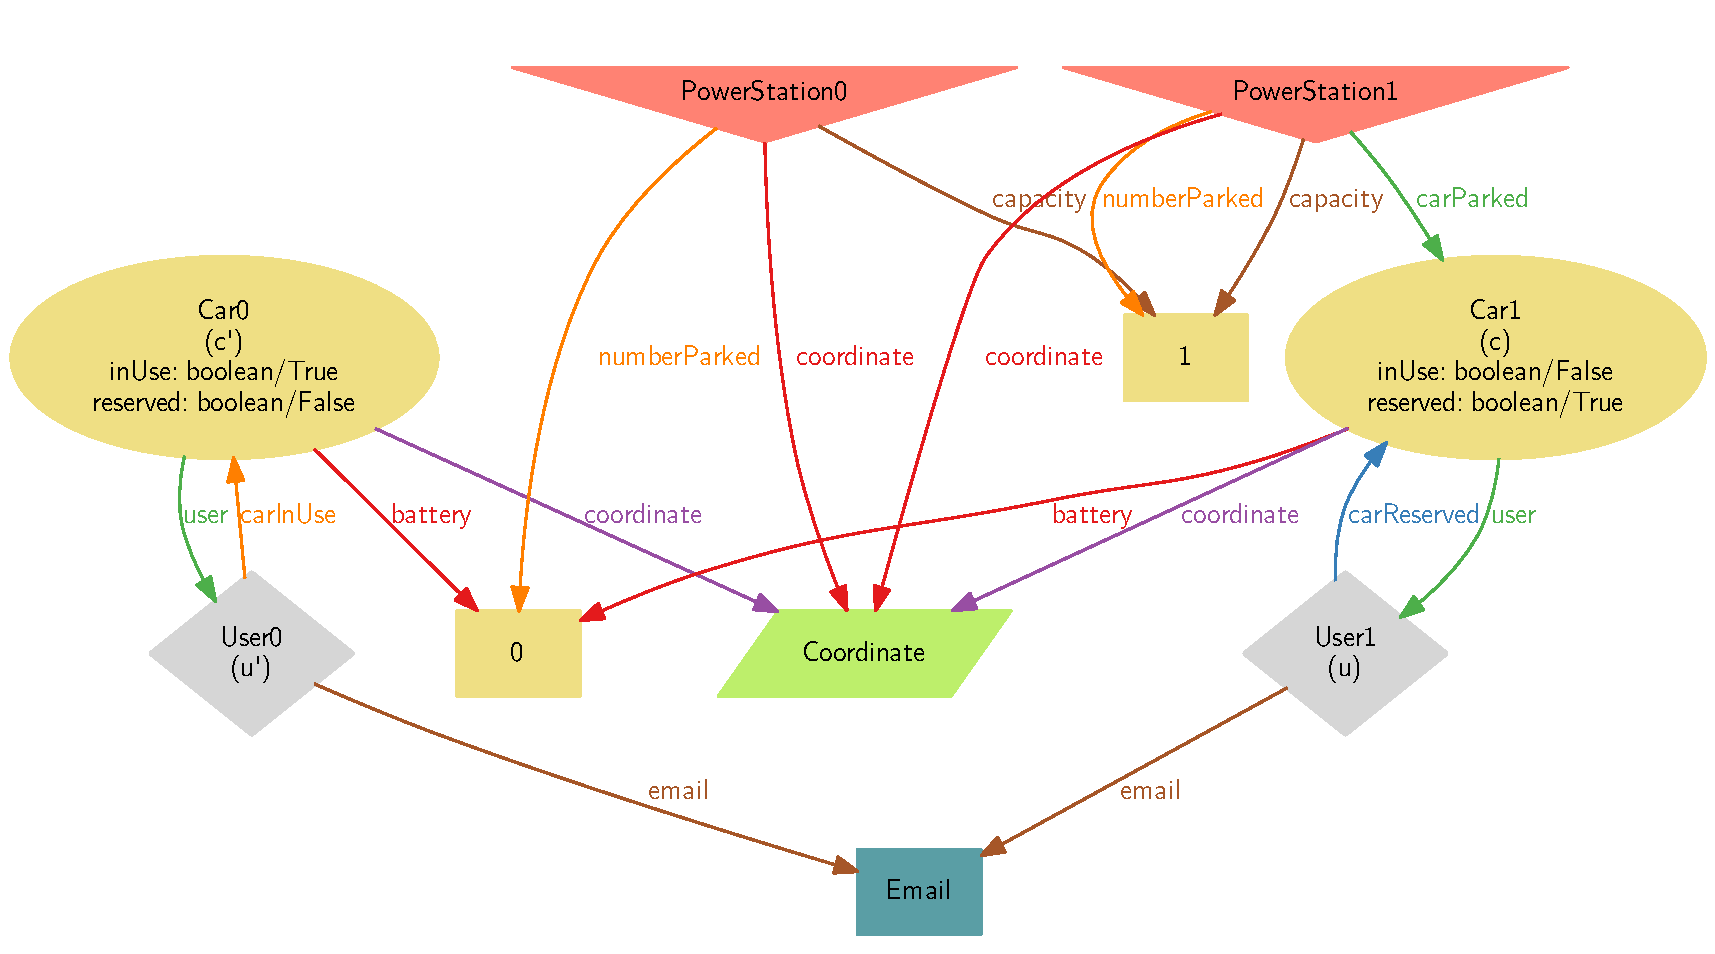
\includegraphics[scale=0.41]{reservedToInUse}\end{textblock}
\par\end{center}
\end{frame}

\section{Design}
\begin{frame}[plain]
\begin{center}
\textbf{\Large{}Design}
\par\end{center}{\Large \par}

\end{frame}
\begin{frame}{Design - Prime scelte}

\begin{textblock}{50}(5,20)
\begin{itemize}[<1->]
\item<1-> Approccio misto Top-down/Bottom-up
\item<2-> Architettura 3 Tier Client-Server con Thin Client:
\begin{itemize}
\item<3-> possibilit� di gestire diversi client
\item<4-> nessuna limitazione sull'hardware dei client
\end{itemize}
\item<5-> Interazioni con componenti esterne
\end{itemize}
\end{textblock}

\begin{textblock}{80}(50,20)

\includegraphics[scale=0.3]{\string"ComponentView - Page 1 (1)\string".pdf}

\end{textblock}

\end{frame}
%
\begin{frame}{I componenti del Server}

\Fontvi

\begin{textblock}{65}(0,12)
\begin{enumerate}
\item \label{G-signUp}Permettere all'utente di registrarsi
\item \label{G-logIn}Permettere all'utente di fare login
\item \label{G-updateProfile}Permettere a utenti aggiornamento e modifica
dei profili.
\item \label{G-updatedInfoOnCars}Mostrare informazioni sulle auto disponibili.
\item \label{G-activeCanReserve}Permettere la prenotazione delle macchine.
\item \label{G-activeCanUnlock} Permettere di sbloccare le macchine.
\item \label{G-computeFare}Calcolare il dovuto.
\item \label{G-sysadminCanUpdate}Permettere agli Admin di aggiornare i
dati del sistema.
\item \label{G-ensureFarePaid}Assicurarsi che i pagamenti vengano effettuati
\item \label{G-driverCanMoneySave}Permettere al guidatore di attivare la
Money Saving Option.
\item \label{G-parkCar}Permettere agli utenti di parcheggiare nelle zone
predeterminate.
\end{enumerate}
\end{textblock}

\begin{textblock}{20}(68,12)\includegraphics[scale=0.29]{\string"ITP - Page 1\string".pdf}\end{textblock}
\end{frame}
%
\begin{frame}{Come e dove mettere i componenti?}
\begin{columns}[c]
\pause

\column{.55\textwidth}
\begin{itemize}
\item Crescente adozione di provider PaaS e affidabilit� delle componenti
di terze parti\pause
\item Architettura a Micro Servizi su Cloud\pause
\begin{itemize}
\item Scalabilit�\pause
\item Indipendenza nello sviluppo\pause
\item Indipendenza nel deployment\pause
\item Indipendenza dall'hardware\pause
\end{itemize}
\item Database centralizzato\pause
\item Necessari alcuni componenti per sfruttare appieno questa scelta architetturale
\end{itemize}

\column{.65\textwidth}

\includegraphics[scale=0.25]{\string"component lvl 2 - Page 1\string".pdf}
\end{columns}

\end{frame}
%
\begin{frame}{La comunicazione}

\begin{textblock}{50}(5,20)
\begin{itemize}[<2->]
\item<2-> Broker di messaggi centralizzato a code Pub/Sub:
\begin{itemize}[<2->]
\item<3-> Possibile singolo punto di rottura
\item<4-> Comunicazione asincrona
\item<5-> Offre funzionalit� di load balancing tra le diverse istanze dei componenti,
anche specifico ``per versione''
\end{itemize}
\end{itemize}
\end{textblock}

\begin{textblock}{50}(55,15)\includegraphics[scale=0.21]{\string"Copy of ComponentDiagramGoals - Page 1\string".pdf}\end{textblock}
\end{frame}
%
\begin{frame}{Il Deployment}

\begin{textblock}{45}(0,20)
\begin{itemize}[<1->]
\item<1-> PowerStation: sistema di acquisizione dati
\item<2-> Automobile: sistema di gestione
\item<3-> Clients:
\begin{itemize}
\item<4-> Mobile App
\item<5-> Web App
\end{itemize}
\item<6-> Schema DBMS
\item<7-> Microservizi
\end{itemize}
\end{textblock}

\begin{textblock}{50}(53,5)

\includegraphics[bb=100bp 0bp 1272bp 1069bp,scale=0.22]{\string"Deployment1 - Page 1\string".pdf}

\end{textblock}

\end{frame}
%
\begin{frame}{Altro}

Nel design document abbiamo poi ulteriormente approfondito:\pause
\begin{itemize}
\item interazioni tra componenti \textrightarrow{} sequence diagram\pause
\item interarfaccia utente \textrightarrow{} UX diagram e mockup\pause
\item struttura del database \textrightarrow{} ER diagram\pause
\item algoritmi: ottimizzazione posizionamento delle auto con MoneySavingOption
\end{itemize}
\end{frame}

\section[Testing]{Test di integrazione}
\begin{frame}[plain]
\begin{center}
\textbf{\Large{}Test di integrazione}
\par\end{center}{\Large \par}

\end{frame}
\begin{frame}{Criteri di ingresso}

Prima di entrare nella fase di integrazione e relativo testing � necessario
che le seguenti condizioni siano verificate.\pause
\begin{itemize}
\item L'\textbf{ambiente} di test deve essere pronto.\pause
\item Tutti i \textbf{test di unit�} devono essere completati.\pause
\item Le \textbf{dipendenze} tra i moduli devono essere definite.\pause
\item Per ogni caso di test devono essere definiti gli \textbf{input} e
i relativi \textbf{output} attesi.\pause
\item Devono essere pronti gli \textbf{stub} delle parti del sistema che
non sono ancora state implementate.
\end{itemize}
\end{frame}
%
\begin{frame}{Strategia di integrazione}

Sono da \textbf{integrare} tutti i moduli mostrati nella fase di design.\pause
\begin{itemize}
\item Abbiamo deciso di utilizzare un approccio \textbf{bottom-up}, cio�
di integrare man mano i componenti che hanno meno dipendenze.\pause
\item In questo modo non � necessaria la creazione di stub, ma solo di \textbf{driver}.\pause
\item Inoltre risulta pi� \textbf{semplice} verificare il comportamento
dei componenti meno integrati testando i componenti di base il \textbf{prima
possibile}.\pause
\item In questo modo tuttavia risulta molto difficile scovare errori nei
componenti che vengono integrati alla fine.\pause
\item Inoltre risulta impossibile vedere l'intero sistema funzionante prima
della fine del processo.
\end{itemize}
\end{frame}

\end{document}
